\documentclass{bmstu}

\bibliography{biblio}

\setenumerate[1]{label=\arabic*.}
\usepackage{listingsutf8}
\lstset{columns=fixed,basicstyle=\small,breaklines=true,inputencoding=utf8,keywordstyle=\bfseries\underbar,frame=single,tabsize=2,xleftmargin=20pt,xrightmargin=5pt}
\lstset{language=sql}
\lstset{numbers=left,numberstyle=\small}
\lstset{xleftmargin=10mm}
\lstset{xrightmargin=-1mm}
\usepackage{mathtools}

\renewcommand\labelitemi{---}
\renewcommand\labelitemii{*}
\renewcommand\labelitemiii{-}

\usepackage{caption}

\lstset{extendedchars=\true}

\usepackage[fontsize=14pt]{fontsize}

\usepackage{pdfpages}

%\usepackage{framed}

%\geometry{
% a4paper,
% left=30mm,
% top=20mm,
% bottom=22mm,
% right=15mm,
% bindingoffset=0cm
% }

\geometry{a4paper,left=3cm,right=1cm,
    top=2cm,bottom=2cm,bindingoffset=0cm}
    
\setlength{\parindent}{1.25cm}
 
 \usepackage{tocloft}

\setlength{\cftbeforetoctitleskip}{0pt}
\renewcommand{\contentsname}{СОДЕРЖАНИЕ}
\renewcommand{\cfttoctitlefont}{\hfill\normalsize\bfseries}
\renewcommand{\cftaftertoctitle}{\hfill\mbox{}}


% Remove padding for TOC entries
\renewcommand{\cftsecindent}{0em}
\renewcommand{\cftsubsecindent}{0em}
\renewcommand{\cftsubsubsecindent}{0em}

% Customizing TOC entries font and alignment
\renewcommand{\cftsecfont}{\normalsize}
\renewcommand{\cftsubsecfont}{\normalsize}
\renewcommand{\cftsubsubsecfont}{\normalsize}

\setlength{\cftbeforetoctitleskip}{-20pt}

\usepackage{indentfirst}

\usepackage{caption} %заголовки плавающих объектов
\captionsetup[table]{justification=centering}

\begin{document}

\includepdf[pages=-]{title.pdf}

%\makethesistitle{Информатика и системы управления}{Программное обеспечение ЭВМ и информационные технологии}{Метод ограничения пропускной способности дискового ввода-вывода в
%системе оркестрации приложений Kubernetes}{А. В. Княжев/ИУ7-82Б}{Ю. В. Строганов}{}{ }

\setcounter{page}{5}

\begin{essay}{}

\textbf{Ключевые слова:} базы данных, языки запросов, Prolog, SQL, ORM.

В данной работе проведен обзор существующих видов запросов в произвольной предметной области, обзор систем управления базами данных PostgreSQL и Greenplum. Кроме того, проведен опрос, позволяющий определить среднее время ответа респондентов и процент ошибок в вопросах, связанных с запросами к базе данных на SQL, Prolog/Datalog и ORM. По результатам опроса выявлено, что вопросы с Prolog/Datalog занимают в среднем меньшее время на заданной выборке респондентов.

\end{essay}

\maketableofcontents

\begin{definitions}
	\definition{Система управления базами данных}{это набор программ, которые управляют структурой БД и контролируют доступ к данным, хранящимся в БД~\cite{швецов2009базы}.}
	\definition{Сериализация}{процесс перевода структуры в текстовый формат, предназначенный для обмена информацией между существенно отличающимися друг от друга программными системами.~\cite{погодин2018сериализация}}
\end{definitions}
\begin{abbreviations}
	\definition{FD}{File Descriptor~\cite{dumitran2007fixing}.}
	\definition{HTTP}{HyperText Transfer Protocol~\cite{fielding2022rfc}.}
	\definition{TCP}{Transmission Control Protocol~\cite{eddy2022rfc}.}
\end{abbreviations}

\chapter*{ВВЕДЕНИЕ}
\addcontentsline{toc}{chapter}{ВВЕДЕНИЕ}

Ежегодно кафедра ИУ7 проводит конкурс «Шаг в будущее» для абитуриентов в соотвествии с положением и регламентом проведения данного конкурса \cite{bib1, bib2}. Конкурс в 2023 году был проведен 24 марта. Организаторы конкурса согласованы в документе состава оргкомитета \cite{bib3}, а также все организационные материалы и члены жюри олимпиады «Шаг в будущее» утверждены в соответствующих документах \cite{bib4, bib5}.

\textbf{Цель практики}~---~организация проектного этапа олимпиады <<Шаг в будущее~---~2023>> МГТУ им. Н.Э. Баумана, секции кафедры ИУ-7 в форме программного салона.

Для достижения поставленной цели необходимо решить следующие задачи.

\begin{enumerate}
	\item Установить ПО, необходимое для демонстрации работы проектов участников.
	\item Изучить работу участников.
	\item Составить студенческие рецензии.
	\item Произвести обзвон участников.
	\item Поучаствовать в очной оценке работ.
\end{enumerate}

\chapter{Аналитический раздел}

\section{Анализ предметной области}
С увеличением числа сотрудников компании часто возникают проблемы внутренней коммуникации сотрудников, получения информации о коллегах и автоматизации процессов рекрутмента~\cite{intranet_avito}. Для решения этих задач существуют внутренние порталы для сотрудников. Обычно они представляют функционал, схожий с соцсетями: отображение профилей пользователей, и др. 

В основном, внутренние порталы для сотрудников представляют собой закрытые решения~\cite{глухих2005глухих}, которые разрабатываются в рамках одной компании~\cite{rivelty}, и не распространяются во внешний мир вследствии политики конфиденциальности~\cite{klee2000importance}. 



\section{Сравнение с аналогичными решениями}
В данной части проводится сравнение предлагаемого решения с аналогами~---~наиболее активно используемыми и разрабатываемыми известными внутренними порталами для сотрудников~\cite{rivelty}.

\paragraph{Критерии сравнения} \mbox{}

В качестве критериев сравнения решений были выбраны основные элементы функционала:

\begin{enumerate}
	\item возможность просматривать профили пользователей;
	\item хранение информации об иерархии сотрудников;
	\item возможность хранить информацию о команде сотрудника;
	\item отсутствие платы за использование;
	\item открытость решения для использования.
\end{enumerate}


\paragraph{Сравнение} \mbox{}

В таблице \ref{table:anal_compare} приведено сравнение решений для внутреннего портала для сотрудников организации.

\begin{table}[h]
  \caption{\label{table:anal_compare} Сравнение существующих решений с предложенным}
  \begin{center}
    \begin{tabular}{|l|l|l|l|l|l|}
      \hline
      Решение              & 1 & 2 & 3 & 4 & 5 \\ \hline
      Интранет VK~\cite{intranet_vk}          & $+$ & $+$ & $-$ & $+$ & $-$ \\ \hline
      Avito People~\cite{intranet_avito}         & $+$ & $+$ & $+$ & $+$ & $-$ \\ \hline
      Битрикс24~\cite{bitrix24}           & $+$ & $+$ & $-$ & $-$ & $+$ \\ \hline
      Предлагаемое решение & $+$ & $+$ & $+$ & $+$ & $+$ \\ \hline
    \end{tabular}
  \end{center}
\end{table}

\section{Формализация задачи}
Решение должно представлять собой портал, в котором будет производиться регистрация сотрудника менеджером по персоналу. Сотрудник сможет просматривать профили других сотрудников, производить поиск по организации.

Каждый сотрудник состоит в некоторой иерархии: у него есть руководитель и подразделение, в котором он находится. Кроме того, роль сотрудника может не совпадать с его положением в этой иерархии~\cite{intranet_avito}. Например, по документам он может находиться в департаменте разработки, а фактически находиться в команде какого-либо проекта. Решение должно учитывать эту особенность.

Сотрудник может редактировать основные данные профиля: фотографию, описание профиля, информацию об отпуске, при этом такую информацию, как имя, должность и положение в иерархии компании может изменять только рекрутер.


\paragraph{Формализация сценариев использования} \mbox{}

В рамках решения должно существовать три вида пользователей:

\begin{enumerate}
	\item Сотрудник~---~сотрудник предприятия. Имеет базовые возможности по изменению части информации профиля, поиску среди пользователей системы.
	\item Рекрутер~---~менеджер по персоналу. Может создавать профили сотрудников, удалять их, изменять базовую информацию, такую как имя, должность.
	\item Администратор~---~главная роль в системе. Может делать то же, что может рекрутер. Кроме того, может редактировать базовую структуру организации, и управлять другими администраторами.
\end{enumerate}

На рис.~\ref{img:use-case} изображена диаграмма сценариев использования предлагаемого решения.

\begin{figure}[h!]
\centering
    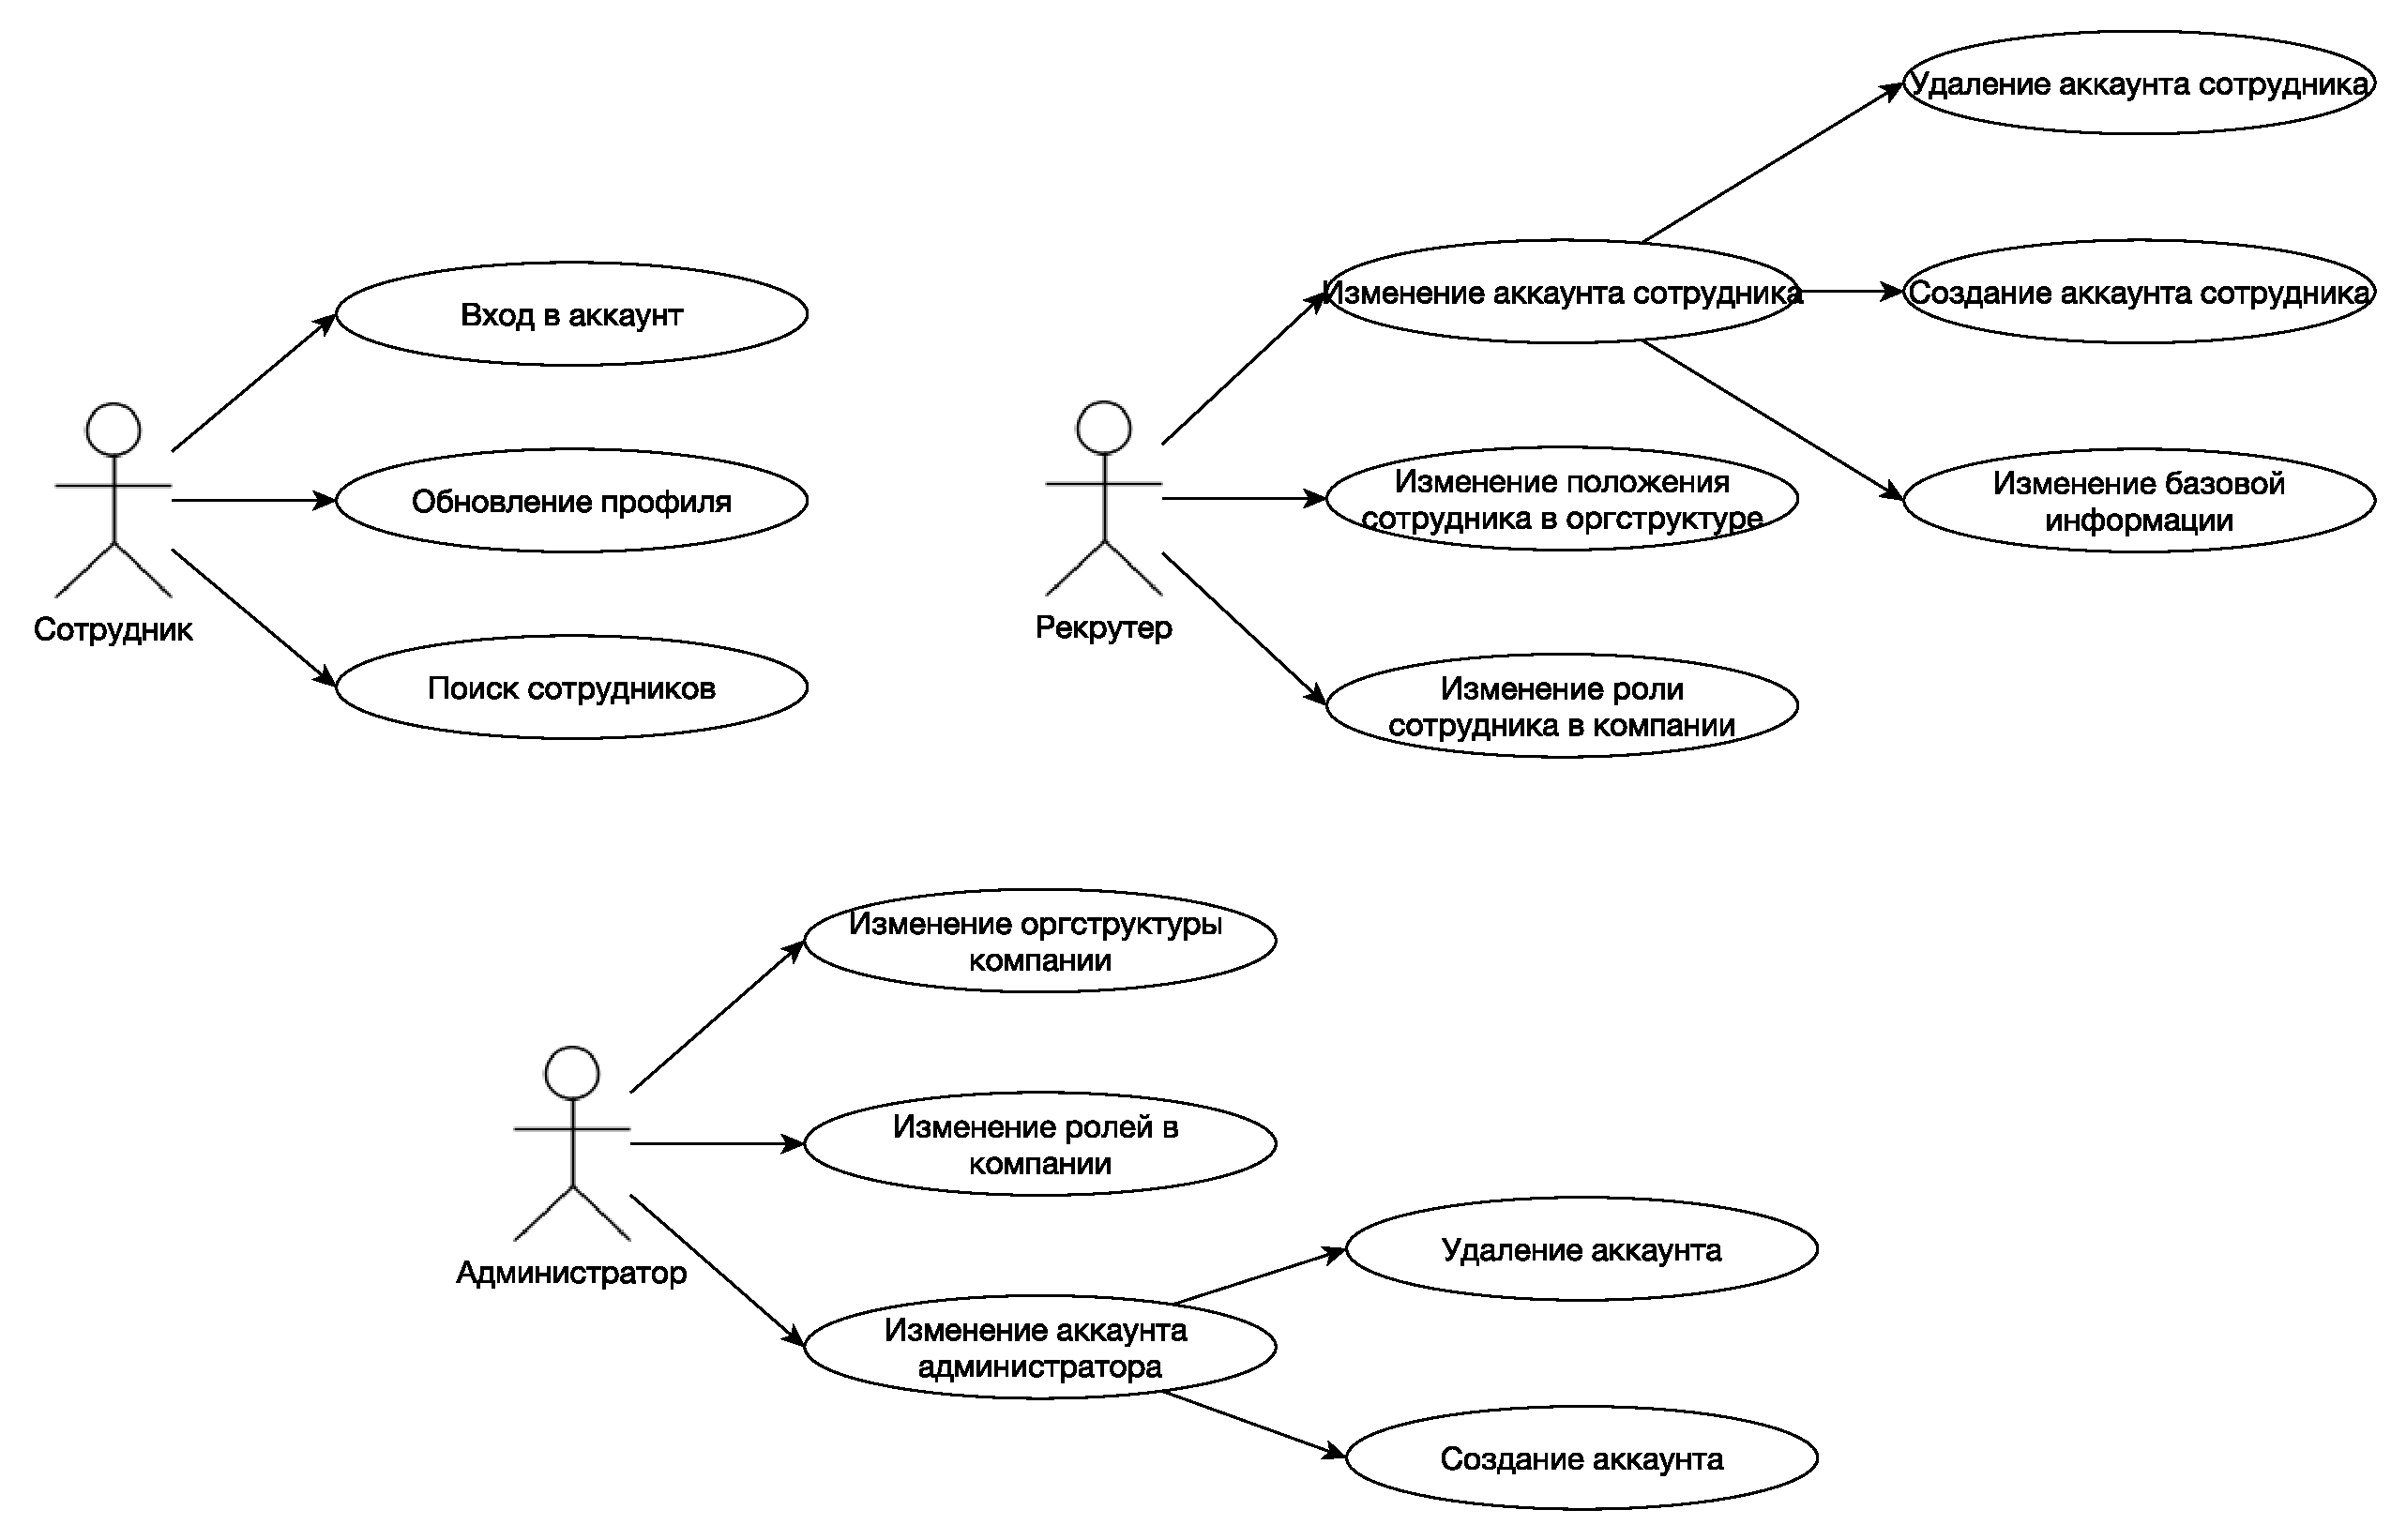
\includegraphics[width=0.9\linewidth]{assets/use-case.pdf}
    \caption{Диаграмма сценариев использования (начало)}
    \label{img:use-case}	
\end{figure}

%\begin{figure}[h!]
%\centering
%    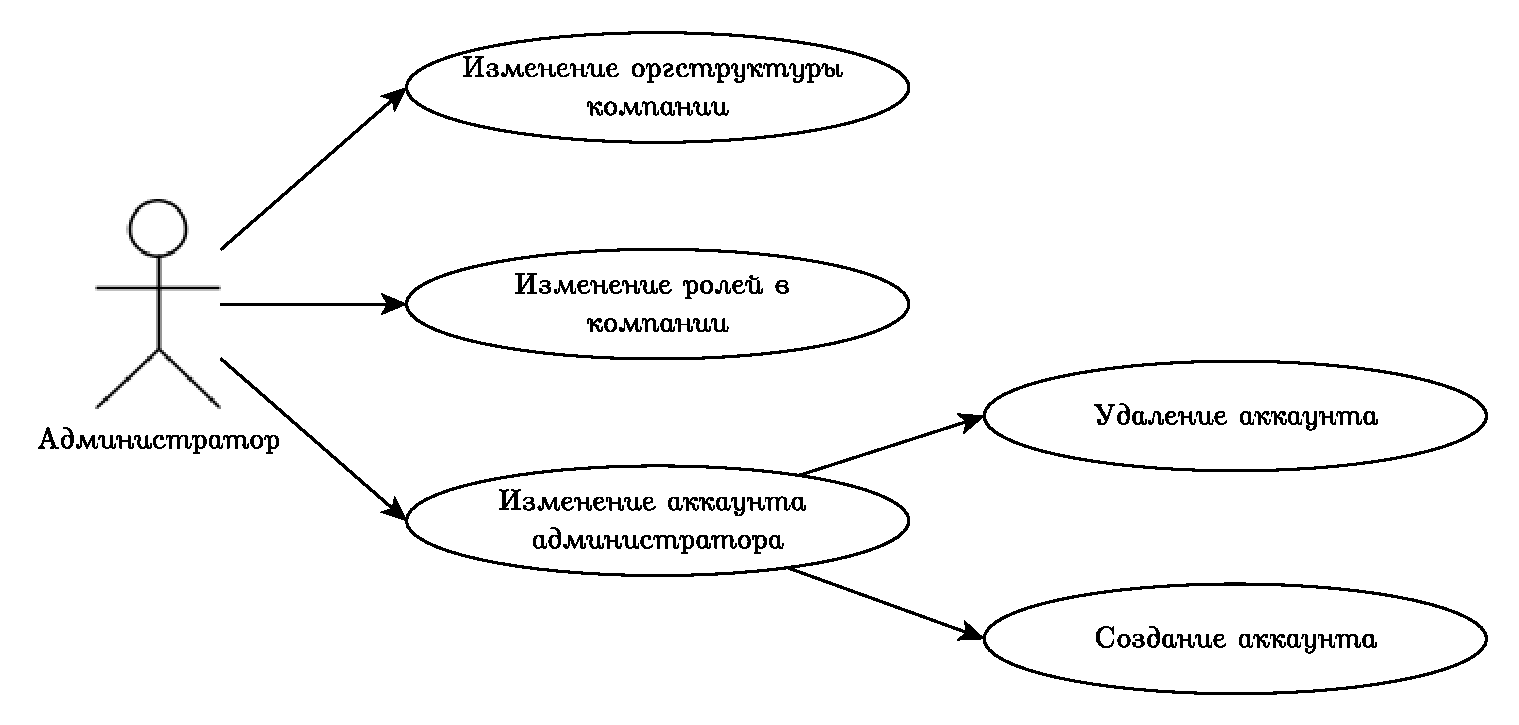
\includegraphics[width=0.8\linewidth]{assets/use-case1.pdf}
%    \caption{Диаграмма сценариев использования (конец)}
%    \label{img:use-case1}	
%\end{figure}


\paragraph{Формализация данных} \mbox{}

Основные сущности, которые должны содержаться в проектируемой базе данных:

\begin{itemize}
	\item сотрудник;
	\item команда~---~фактическая команда, в которой работает сотрудник;
	\item подписка;
	\item отпуск;
	\item отдел~---~официальный департамент, в который трудоустроен сотрудник.
\end{itemize}

На рис.~\ref{img:chen} изображена ER-диаграмма сущностей проектируемой базы данных в нотации Чена.

\newpage

\begin{figure}[h!]
\centering
    \includegraphics[width=0.9\linewidth]{assets/chen.pdf}
    \caption{ER-диаграмма сущностей в нотации Чена}
    \label{img:chen}	
\end{figure}


\section{Виды СУБД по модели данных}

База данных представляет собой набор связанных данных некоторой предметной области, поэтому для ее организации важно определиться с моделью данных. Модель данных представляет собой логическую структуру данных, хранящихся в базе данных~\cite{хомоненко2000базы}. На данный момент, в качестве основных моделей данных выделяют дореляционные, реляционные и нереляционные.

\paragraph{Дореляционные} \mbox{}

Дореляционные базы данных не основываются на абстрактных моделях, доступ осуществляется на уровне записей~\cite{бородин2016задаче}. 

Среди дореляционных моделей можно выделить~\cite{дадян2016методы}:
\begin{itemize}
	\item Иерархическая~---~представлена в базе данных в виде дерева~\cite{корягин2020модели}.
	\item Сетевая~---~является расширением иерархической БД. У потомка может быть больше одного родителя. Такая модель поддерживает отношение «многие-ко-многим»~\cite{корягин2020модели}. 
\end{itemize}

Среди особенностей дореляционных моделей можно отметить сложность использование и зависимость прикладных программ от физической реализации СУБД~\cite{бородин2016задаче}. 

\paragraph{Реляционные} \mbox{}

Реляционная база данных~---~совокупность отношений, содержащих всю информацию, которая должна храниться в базе данных~\cite{кириллов2012введение}. В основном воспринимаются как базы, в которых данные хранятся в двумерных таблицах, а установленная между ними связь позволяет избегать повторения данных~\cite{жалолов2020понятие}.


Таблица реляционной базы данных устроена следующим образом. Столбец таблицы представляет собой поле~---~значение атрибута отношения. Строка представляет собой конкретную запись, кортеж этого отношения. Такая структура позволяет создать наиболее простое и понятное пользователю представление базы данных, при такой организации данные хорошо структурированы~\cite{бородин2016задаче}. 


\paragraph{Нереляционные} \mbox{}

Нереляционные модели убирают строгие связи между данными в системе. Нереляционные базы данных бывают~\cite{бородин2016задаче}:

\begin{itemize}
	\item колоночные;
	\item документоориентированные;
	\item вида ключ-значение;
	\item графовые;
	\item с другие.
\end{itemize}

Основными отличиями от реляционной модели являются меньшая структуризация, отсутствие стандартизации~\cite{корягин2020модели}.

В данном разделе была проведена формализация задачи: рассмотрена предметная область, формализованы данные и сценарии использования. Проведено сравнение с конкурентами по основным критериям.

Кроме того, рассмотрены виды СУБД по модели данных. В связи с отсутствием необходимости специфичной обработки данных и необходимостью структурировать данные, была выбрана реляционная модель.

 
\chapter{Проведение конкурса}

\section{Оценка по результатам очной проверки}
Для дальнейшей оценки студенческого жюри необходимо внимательно изучить работы участников конкурса и заполнить таблицы с баллами. Для этого все студенты-организаторы разбиваются на группы по 2 человека, чтобы оценить всех абитуриентов.

Сначала происходит ознакомление с докладом автора, опрос по теме выступления. Далее необходимо оценить в работе следующее:

\begin{enumerate}
	\item структуру и оформление работы;
	\item актуальность тематики работы;
	\item полноту раскрытия темы;
	\item логику изложения, оригинальность мышления;
	\item используемые методы и обоснование их использования;
	\item наличие в тексте работы заимствований из источников, в том числе из ресурсов сети Интернет;
	\item наличие предложений по практическому использованию программы;
	\item вклад автора в выбранную тему.
\end{enumerate}

Работая в группе с Екатериной Карповой, мы просмотрели и оценили 6 работ абитуриентов.

Была составлена результирующая таблица с оценками участников, со стороны как студенческого, так и преподавательского жюри. После подсчета набранных участниками конкурса баллов, были определены три победителя этапа олимпиады «Шаг в будущее» и один участник, выбранный студенческим жюри. Призерам была вручена научная литература, выпущенная в издательстве МГТУ им. Н.Э. Баумана.


\section{Сведения об участнике и работе}

Студенческому жюри были представлены работы участников конкурса, после чего была произведена их оценка. Далее будет представлен анализ одной из работ.

Рассматриваемая далее работа была выполнена Решетниковым Федором Владимировичем, учеником ГБОУ Инженерная Школа 1581. Тема работы, представленная им на конкурсе: «Создание сервиса для определения оптимального времени для проведения события».

По словам участника, цель работы~---~<<сделать приложение для оптимизации выбора группой времени для встречи или событий, с учётом желаний потенциальных пользователей.>>

Участник утверждает: <<Во время карантина 2021 года компании и команды стали работать удалённо и виделись через камеру. После огромное количество команд осталось работать удалённо, не требует затрат на офис, да и все успели привыкнуть. В таких условиях еще больше участились случаи когда нужно в онлайн договориться, когда провести созвон или любое другое событие.  Например команде стартапа нужно решить, когда провести созвон, вне расписания, что бывает довольно часто. Или работникам компании с плотным графиком, нужно разобраться, когда лучше провести совещание. Также это может быть нужно даже вне работы например сбор бывших одноклассников на встречу или друзей на день рождения. Чисто переписываться муторно и долго, т.к. о времени все могут писать по-разному, а считать всё нужно в ручную.>> Орфография и пунктуация автора сохранены.

Заявлена следующая работа ПО: совместное планирование событий, создание ссылок на события.

\begin{table}[h!]
  \centering
  \begin{tabular}{p{1\linewidth}}
    \centering
    \includegraphics[width=1\linewidth]{./images/example.pdf}
    \captionof{figure}{Пример работы ПО}
    \label{img:func}
  \end{tabular}
\end{table}

\newpage

\section{Результаты очной проверки}

Большая часть работы не была выполнена самим участником (CI/CD, бекенд были сделаны не участником). Актуальность работы не обоснована, не рассмотрены такие очевидные аналоги, как Google Calendar. На защите участник не ориентировался в коде. РПЗ содержит огромное количество орфографических, грамматических, лексических и пунктуационных ошибок, не выдержан стиль речи.

\newpage
\chapter{Технологический раздел}

В качестве языка программирования для реализации разработанного метода был выбран Go~\cite{donovan2015go}, так как с помощью него можно решить поставленную задачу, а также он имеет достаточный набор библиотек для взаимодействия с Kubernetes. Наличие библиотек также вызвано официальной поддержкой языка Go авторами оркестратора, так как сама система оркестрации реализована с использованием этого языка~\cite{kubernetes}.

Для реализации разрабатываемого ПО был использован паттерн <<Оператор>>, так как он является рекомендуемым для разработки расширений для Kubernetes~\cite{operator}.

Для реализации Kubernetes-оператора использовался Operator SDK, так как он предоставляет достаточный набор функций для создания операторов, в том числе~\cite{operator_sdk}:

\begin{itemize}
	\item генерация шаблона проекта;
	\item генерация обработчиков обновления Custom Resources;
	\item генерация средств развертывания приложения в Kubernetes;
	\item набор библиотек для взаимодействия с Kubernetes.
\end{itemize}

Таким образом, Kubernetes-оператор представляет собой единое приложение, запускающее в себе набор циклов-контроллеров, реагирующих на изменение Custom Resource.

\newpage

На рисунке~\ref{img:po} представлена схема взаимодействия оператора с компонентами Kubernetes и ядра операционной системы Linux.

\begin{figure}[h!]
    \centering
    \includegraphics[width=\textwidth]{assets/po}
    \caption{Схема взаимодействия оператора с компонентами Kubernetes и ядра операционной системы Linux}
    \label{img:po}
\end{figure}

\section{Входные данные}

Входными данными являются сущности Kubernetes. При этом используются три возможных варианта сущностей: Pod, IOLimit, PodIOLimit. При этом Pod является стандартным ресурсом Kubernetes, а IOLimit и PodIOLimit~---~Custom Resource.

\textbf{IOLimit}

Сущность IOLimit хранит информацию об ограничениях дискового ввода-вывода на уровне группы реплик приложения. Манифест этого ресурса имеет вид, представленный в листингах~\ref{lst:iolimit1}--\ref{lst:iolimit2}.

\begin{lstlisting}[label=lst:iolimit1, caption={Пример манифеста IOLimit}]
apiVersion: ioba.dbaas.avito.ru/v1alpha1
\end{lstlisting}

\begin{lstlisting}[label=lst:iolimit2, caption={Пример манифеста IOLimit (продолжение листинга~\ref{lst:iolimit1})}]
kind: IOLimit
metadata:
  name: test-limit
spec:
  storageName: db1
  replicaSetName: rs001
  containers:
    - name: postgresql
      volumes:
        - name: data
          reads:
            iops: 300
            bandwidth: 100MBps
          writes:
            iops: 300
            bandwidth: 20MBps
\end{lstlisting}

При создании или изменении сущности IOLimit, оператор дозаполнит необходимую низкоуровневую информацию и создаст ресурсы PodIOLimit для каждого экземпляра Pod.      

\textbf{Pod}

Так как может быть такая ситуация, что некоторые поды, относящиеся к приложению будут созданы после применения ограничений на существующие поды хранилища, то необходимо отслеживать создание новых подов, и в случае несуществования для них подходящих ресурсов PodIOLimit создавать их.

\textbf{PodIOLimit}

Сущность PodIOLimit хранит информацию об ограничениях дискового ввода-вывода на уровне одной реплики приложения. Манифест этого ресурса имеет вид, представленный в листингах~\ref{lst:podiolimit1}--\ref{lst:podiolimit2}.

\begin{lstlisting}[label=lst:podiolimit1, caption={Пример манифеста PodIOLimit}]
apiVersion: ioba.dbaas.avito.ru/v1alpha1
kind: PodIOLimit
metadata:
  name: test-limit-ioba-test-0
spec:
\end{lstlisting}

\begin{lstlisting}[label=lst:podiolimit2, caption={Пример манифеста PodIOLimit (продолжение листинга~\ref{lst:podiolimit1})}]
  limits:
    - containerID: bb6deeaa978e99a
      containerName: postgresql
      deviceNumbers: "254:1"
      readBandwidth: "100000000"
      readIOPS: "300"
      volumeName: data
      writeBandwidth: "20000000"
      writeIOPS: "300"
  nodeName: worker2
  podName: test-0
  podUID: 9b06e0ab-fd1f-49b9-8581-d4eed47b282a
  replicaSetName: rs001
  storageName: db1
\end{lstlisting}

\section{Создание PodIOLimit на основе IOLimit}

Кроме информации непосредственно из IOLimit, PodIOLimit для каждого контейнера имеет набор системной информации, такой как идентификатора пода и контейнера, и номера примонтированного устройства. Соответственно, для генерации PodIOLimit необходимо получить эту низкоуровневую информацию.

Идентификатор пода содержится в его метаданных. Листинги~\ref{lst:pod_uid1}--\ref{lst:pod_uid2} содержат фрагмент кода, получающий идентификатор пода.

\begin{lstlisting}[language=Go,label=lst:pod_uid1, caption={Получение идентификатора пода}]
podLimit := &dbaasv1alpha1.PodIOLimit{
	ObjectMeta: metav1.ObjectMeta{
		Name:       fmt.Sprintf("%s-%s", iolimit.Name, pod.Name),
		Namespace:  pod.Namespace,
		Finalizers: []string{dbaasv1alpha1.CleanupFinalizer},
		Labels: map[string]string{
			dbaasv1alpha1.NodeNameLabel: g.nodeName,
		},
	},
	Spec: dbaasv1alpha1.PodIOLimitSpec{
\end{lstlisting}

\begin{lstlisting}[language=Go,label=lst:pod_uid2, caption={Получение идентификатора пода (продолжение листинга~\ref{lst:pod_uid1})}]
		StorageName:    iolimit.Spec.StorageName,
		ReplicaSetName: iolimit.Spec.ReplicaSetName,
		Limits:         limits,
		NodeName:       g.nodeName,
		PodName:        pod.Name,
		PodUID:         string(pod.UID),
		},
}
\end{lstlisting}

Идентификатор контейнера получается из информации о состоянии пода. Листинги~\ref{lst:container_id1}--\ref{lst:container_id2} содержат фрагмент кода получения идентификатора контейнера.

\begin{lstlisting}[language=Go,label=lst:container_id1, caption={Получение идентификатора контейнера}]
func (g *Generator) prepareLimits(pod *v1.Pod, iolimit *dbaasv1alpha1.IOLimit) ([]models.LimitBase, error) {
	volumeToPVC := make(map[string]string, len(pod.Spec.Volumes))
	for _, volume := range pod.Spec.Volumes {
		if volume.PersistentVolumeClaim == nil {
			continue
		}

		volumeToPVC[volume.Name] = volume.PersistentVolumeClaim.ClaimName
	}

	containerNameToID := make(map[string]string, len(pod.Spec.Containers))
	for _, status := range pod.Status.ContainerStatuses {
		containerNameToID[status.Name] = g.trimCRIPrefix(status.ContainerID)
	}

	limits := make([]models.LimitBase, 0, len(iolimit.Spec.Containers))
	for _, container := range iolimit.Spec.Containers {
		for _, volume := range container.Volumes {
\end{lstlisting}

\begin{lstlisting}[language=Go,label=lst:container_id2, caption={Получение идентификатора контейнера (продолжение листинга~\ref{lst:container_id1})}]
			pvc, ok := volumeToPVC[volume.Name]
			if !ok {
				return nil, fmt.Errorf("get pvc by volume: %w", models.ErrPVCNotFound)
			}

			containerID, ok := containerNameToID[container.Name]
			if !ok || containerID == "" {
				return nil, fmt.Errorf("get container id by name: %w", models.ErrContainerNotFound)
			}

			limits = append(limits, models.LimitBase{
				Namespace:     iolimit.Namespace,
				PodUID:        string(pod.UID),
				ContainerName: container.Name,
				ContainerID:   containerID,
				VolumeName:    volume.Name,
				PVCName:       pvc,
				Reads:         volume.Reads,
				Writes:        volume.Writes,
			})
		}
	}

	return limits, nil
}
\end{lstlisting}


Фрагмент получения номеров устройства из файловой системы proc представлен в листингах~\ref{lst:proc_parse1}--\ref{lst:proc_parse2}.

\begin{lstlisting}[language=Go,label=lst:proc_parse1, caption={Получение номеров устройства}]
func (e *Extractor) DeviceNumbers(
    ctx context.Context, 
    containerPID int, 
    volumeHandle string,
\end{lstlisting}

\newpage

\begin{lstlisting}[language=Go,label=lst:proc_parse2, caption={Получение номеров устройства (продолжение листинга~\ref{lst:proc_parse1})}]
) (string, error) {
	file, err := e.reader.Read(filepath.Join(strconv.Itoa(containerPID), "mountinfo"))
	if err != nil {
		return "", fmt.Errorf("read proc file: %w", err)
	}
	deviceNumbers, err := e.deviceNumberFromMountInfo(file, volumeHandle)
	if err != nil {
		return "", fmt.Errorf("extract device numbers: %w", err)
	}
	
	return deviceNumbers, nil
}

func (e *Extractor) deviceNumberFromMountInfo(mountInfo, volumeHandle string) (string, error) {
	for _, line := range strings.Split(mountInfo, "\n") {
		if !strings.Contains(line, volumeHandle) {
			continue
		}
		splitted := strings.Split(line, " ")
		if len(splitted) < deviceNumbersColumn {
			return "", fmt.Errorf("line must contain more than 3 columns: %w (%q)", models.ErrInvalidProcFile, line)
		}
		return splitted[deviceNumbersColumn-1], nil
	}

	return "", fmt.Errorf("mount not found for volumehandle %s: %w", volumeHandle, models.ErrNoVolumeEntry)
}
\end{lstlisting}

Фрагмент кода получения PID основного процесса контейнера представлен в листинге~\ref{lst:pid}.

\newpage

\begin{lstlisting}[language=Go,label=lst:pid, caption={Получение PID основного процесса контейнера}]
func (e *Extractor) ContainerPID(ctx context.Context, containerID string) (int, error) {
	resp, err := e.cri.ContainerStatus(ctx, containerID, true)
	if err != nil {
		return 0, fmt.Errorf("call containerStatus: %w", err)
	}
	infoMarshalled, ok := resp.Info["info"]
	if !ok {
		return 0, fmt.Errorf("container info response must contain info block: %w", models.ErrInvalidContainerInfo)
	}

	var info containerInfo
	if err := json.Unmarshal([]byte(infoMarshalled), &info); err != nil {
		return 0, fmt.Errorf("unmarshal container info: %w", err)
	}

	if info.PID == 0 {
		return 0, fmt.Errorf("extract container pid: %w", models.ErrInvalidContainerInfo)
	}

	return info.PID, nil
}

type containerInfo struct {
	PID int `json:"pid"`
}
\end{lstlisting}

На основе всех полученных данных может быть сгенерирован PodIOLimit. Фрагмент кода по генерации PodIOLimit представлен в Приложении~Б.

\section{Применение ограничений дискового ввода-вывода с использованием cgroup v2}

Применение ограничений дискового ввода-вывода представляет собой запись в интерфейсный файл \texttt{io.max} контрольной группы контейнера. Фрагмент кода с записью ограничений в файл представлен в листинге~\ref{lst:write_limit}.

\begin{lstlisting}[language=Go,label=lst:write_limit, caption={Запись ограничений в cgroup v2}]
func (w *LimitWriter) WriteLimit(ctx context.Context, podUID string, limit dbaasv1alpha1.Limit) error {
	fileName := w.path.Format(podUID, limit, ioMaxFileName)
	line := w.toCGroupLine(limit)

	if err := w.writer.Write(fileName, line); err != nil {
		return fmt.Errorf("write limit to file: %w", err)
	}

	return nil
}

func (w *LimitWriter) toCGroupLine(limit dbaasv1alpha1.Limit) string {
	return fmt.Sprintf("%s rbps=%s wbps=%s riops=%s wiops=%s",
		w.deviceNumbersGenerator.Generate(limit.DeviceNumbers),
		limit.ReadBandwidth,
		limit.WriteBandwidth,
		limit.ReadIOPS,
		limit.WriteIOPS,
	)
}
\end{lstlisting}

\section{Тестирование}

Для тестирования ПО были реализованы полностью автоматизированные модульные и интеграционные тесты, и частично автоматизированные функциональные тесты. Суммарное тестовое покрытие составляет 89\%. Кроме того, была измерена оценка по мутационному тестированию с использованием утилиты \texttt{go-mutesting}~\cite{mutesting}, полученная оценка равна 86\%.

Пример модульного теста представлен в Приложении~В.

Пример интеграционного теста представлен в приложении~Г.

\chapter{Исследовательский раздел}

Был проведен одновременный тест производительности трех экземпляров системы управления базами данных PostgreSQL без ограничений дискового ввода-вывода и с ограничениями. Результатами исследования является количество транзакций в секунду на трех экземплярах для двух тестовых случаев:

\begin{enumerate}
	\item ввод-вывод не ограничен;
	\item ввод-вывод ограничен на всех экземплярах.
\end{enumerate}

Характеристики оборудования, на которых производились замеры следующие.

\begin{itemize}
\item Процессор: Apple M1 Pro~\cite{mac}.
\item Объем оперативной памяти: 16ГБ~\cite{mac}.	
\end{itemize}

Каждый экземпляр PostgreSQL запускался в отдельном контейнере в Kubernetes, для каждого контейнера были выделены следующие ограничения.

\begin{itemize}
\item Процессорное время: 2 единицы~\cite{resource_management}.
\item Объем оперативной памяти: 3ГБ.	
\end{itemize}

Манифест запуска экземпляров PostgreSQL представлен в Приложении~Д.

Манифест с ограничениями дискового ввода-вывода экземпляров представлен в Приложении~Е.

Для теста производительности использовалась утилита \texttt{pgbench}. Для тестирования вызывался \texttt{pgbench} с параметрами, показанными в листинге~\ref{lst:pgbench}.

\begin{lstlisting}[language=Go,label=lst:pgbench, caption={Параметры pgbench}]
pgbench -i -s 100
pgbench  -c 8 -j 2 -T 120
\end{lstlisting}

\section{Результаты}

Было проведено 10 замеров. Результаты измерений без ограничений дискового ввода-вывода представлены в таблице~\ref{tab:res_without}.


\begin{table}[H]
\caption{Результаты измерений без ограничений дискового ввода-вывода}
\label{tab:res_without}
\begin{center}
\begin{tabular}{|l|r|r|r|}
\hline
\multicolumn{1}{|c|}{\textbf{№ замера}} & \multicolumn{1}{c|}{\textbf{\begin{tabular}[c]{@{}c@{}}Экземпляр 1, \\ TPS\end{tabular}}} & \multicolumn{1}{c|}{\textbf{\begin{tabular}[c]{@{}c@{}}Экземпляр 2, \\ TPS\end{tabular}}} & \multicolumn{1}{c|}{\textbf{\begin{tabular}[c]{@{}c@{}}Экземпляр 3, \\ TPS\end{tabular}}} \\ \hline
1                                       & 1590                                                                                      & 1565                                                                                      & 1622                                                                                      \\ \hline
2                                       & 1625                                                                                      & 1619                                                                                      & 1599                                                                                      \\ \hline
3                                       & 1474                                                                                      & 1481                                                                                      & 1509                                                                                      \\ \hline
4                                       & 1645                                                                                      & 1694                                                                                      & 1668                                                                                      \\ \hline
5                                       & 1406                                                                                      & 1432                                                                                      & 1564                                                                                      \\ \hline
6                                       & 1584                                                                                      & 1534                                                                                      & 1503                                                                                      \\ \hline
7                                       & 1563                                                                                      & 1571                                                                                      & 1497                                                                                      \\ \hline
8                                       & 1528                                                                                      & 1493                                                                                      & 1431                                                                                      \\ \hline
9                                       & 1475                                                                                      & 1762                                                                                      & 1731                                                                                      \\ \hline
10                                      & 1683                                                                                      & 1671                                                                                      & 1697                                                                                      \\ \hline
\end{tabular}
\end{center}
\end{table}


\newpage

Результаты измерений c ограничениями дискового ввода-вывода представлены в таблице~\ref{tab:res_with}.

\begin{table}[H]
\caption{Результаты измерений с ограничениями дискового ввода-вывода}
\label{tab:res_with}
\begin{center}
\begin{tabular}{|l|r|r|r|}
\hline
\multicolumn{1}{|c|}{\textbf{№ замера}} & \multicolumn{1}{c|}{\textbf{\begin{tabular}[c]{@{}c@{}}Экземпляр 1, \\ TPS\end{tabular}}} & \multicolumn{1}{c|}{\textbf{\begin{tabular}[c]{@{}c@{}}Экземпляр 2, \\ TPS\end{tabular}}} & \multicolumn{1}{c|}{\textbf{\begin{tabular}[c]{@{}c@{}}Экземпляр 3, \\ TPS\end{tabular}}} \\ \hline
1                                       & 1569                                                                                      & 1542                                                                                      & 1597                                                                                      \\ \hline
2                                       & 1570                                                                                      & 1592                                                                                      & 1566                                                                                      \\ \hline
3                                       & 1539                                                                                      & 1562                                                                                      & 1601                                                                                      \\ \hline
4                                       & 1585                                                                                      & 1602                                                                                      & 1573                                                                                      \\ \hline
5                                       & 1551                                                                                      & 1608                                                                                      & 1531                                                                                      \\ \hline
6                                       & 1568                                                                                      & 1533                                                                                      & 1584                                                                                      \\ \hline
7                                       & 1524                                                                                      & 1581                                                                                      & 1597                                                                                      \\ \hline
8                                       & 1597                                                                                      & 1540                                                                                      & 1539                                                                                      \\ \hline
9                                       & 1580                                                                                      & 1539                                                                                      & 1602                                                                                      \\ \hline
10                                      & 1556                                                                                      & 1571                                                                                      & 1588                                                                                      \\ \hline
\end{tabular}
\end{center}
\end{table}


Результаты измерений представлены в формате гистограммы на рисунке~\ref{img:plot}.

\begin{figure}[h!]
    \centering
    \includegraphics[width=\textwidth]{assets/plot.jpeg}
    \caption{Гистограмма с результатами бенчмарка}
    \label{img:plot}
\end{figure}

На основании полученных результатов, для двух групп тестов были посчитаны выборочное среднее $\hat{\mu}$, размах выборки $R$ и выборочная дисперсия $\hat{\sigma}^2$. Значения округлены до целых. Результаты подсчетов приведены в таблице~\ref{tab:vlasou}.

\begin{table}[H]
\caption{Размах, выборочное среднее и выборочная дисперсия}
\label{tab:vlasou}
\begin{center}
\begin{tabular}{|l|r|r|}
\hline
                 & \multicolumn{1}{c|}{\textbf{Без ограничений}} & \multicolumn{1}{c|}{\textbf{С ограничениями}} \\ \hline
$\hat{\mu}$      & 1573                                          & 1569                                          \\ \hline
$R$              & 356                                           & 84                                            \\ \hline
$\hat{\sigma}^2$ & 8816                                          & 631                                           \\ \hline
\end{tabular}
\end{center}
\end{table}

В тестовом случае с ограниченным дисковым вводом-выводом выборочная дисперсия и размах выборки меньше, чем в случае без ограничений. На основании этого можно сделать вывод о том, что ограничения дискового ввода-вывода могут обеспечить более стабильную производительность СУБД.

\chapter*{ЗАКЛЮЧЕНИЕ}
\addcontentsline{toc}{chapter}{ЗАКЛЮЧЕНИЕ}

В рамках выполнения работы была разработана база данных внутреннего портала для сотрудников организации. Все поставленные задачи были выполнены:

\begin{itemize}
	\item формализована задача;
	\item спроектирована база данных;
	\item выбрана СУБД;
	\item реализована база данных;
	\item база данных заполнена данными;
	\item реализовано приложение для доступа к базе данных.
\end{itemize}

Цель работы~---~разработка базы данных внутренного портала для сотрудников предприятия, и приложения, позволяющего взаимодействовать с ней, была достигнута.

\makebibliography

\begin{appendices}

\chapter{Интерфейсные файлы контрольной группы}

Пример содержания каталога для контрольной группы представлен в листингах~\ref{lst:cgroup_catalog1}--\ref{lst:cgroup_catalog2}.

\begin{lstlisting}[label=lst:cgroup_catalog1, caption={Интерфейсные файлы для контрольной группы}]
-r--r--r--  1 root root 0 Mar 27 21:40 cgroup.controllers
-r--r--r--  1 root root 0 Mar 27 21:40 cgroup.events
-rw-r--r--  1 root root 0 Mar 27 21:40 cgroup.freeze
--w-------  1 root root 0 Mar 27 21:40 cgroup.kill
-rw-r--r--  1 root root 0 Mar 27 21:40 cgroup.max.depth
-rw-r--r--  1 root root 0 Mar 27 21:40 cgroup.max.descendants
-rw-r--r--  1 root root 0 Mar 27 21:40 cgroup.procs
-r--r--r--  1 root root 0 Mar 27 21:40 cgroup.stat
-rw-r--r--  1 root root 0 May 26 16:54 cgroup.subtree_control
-rw-r--r--  1 root root 0 Mar 27 21:40 cgroup.threads
-rw-r--r--  1 root root 0 Mar 27 21:40 cgroup.type
-rw-r--r--  1 root root 0 Mar 28 18:10 cpu.idle
-rw-r--r--  1 root root 0 Mar 27 21:46 cpu.max
-rw-r--r--  1 root root 0 Mar 28 18:10 cpu.max.burst
-rw-r--r--  1 root root 0 Mar 27 21:40 cpu.pressure
-r--r--r--  1 root root 0 Mar 27 21:40 cpu.stat
-rw-r--r--  1 root root 0 Mar 28 18:10 cpu.uclamp.max
-rw-r--r--  1 root root 0 Mar 28 18:10 cpu.uclamp.min
-rw-r--r--  1 root root 0 Mar 27 21:46 cpu.weight
-rw-r--r--  1 root root 0 Mar 28 18:10 cpu.weight.nice
-rw-r--r--  1 root root 0 Mar 27 21:46 cpuset.cpus
-r--r--r--  1 root root 0 Mar 28 18:10 cpuset.cpus.effective
-rw-r--r--  1 root root 0 Mar 28 18:10 cpuset.cpus.partition
-rw-r--r--  1 root root 0 Mar 27 21:46 cpuset.mems
-r--r--r--  1 root root 0 Mar 28 18:10 cpuset.mems.effective
-r--r--r--  1 root root 0 Mar 28 18:10 hugetlb.1GB.current
-r--r--r--  1 root root 0 Mar 28 18:10 hugetlb.1GB.events
-r--r--r--  1 root root 0 Mar 28 18:10 hugetlb.1GB.events.local
-rw-r--r--  1 root root 0 Mar 28 18:10 hugetlb.1GB.max
-r--r--r--  1 root root 0 Mar 28 18:10 hugetlb.1GB.rsvd.current
-rw-r--r--  1 root root 0 Mar 28 18:10 hugetlb.1GB.rsvd.max
\end{lstlisting}

\begin{lstlisting}[label=lst:cgroup_catalog2, caption={Интерфейсные файлы для контрольной группы (продолжение листинга~\ref{lst:cgroup_catalog1})}]
-r--r--r--  1 root root 0 Mar 28 18:10 hugetlb.2MB.current
-r--r--r--  1 root root 0 Mar 28 18:10 hugetlb.2MB.events
-r--r--r--  1 root root 0 Mar 28 18:10 hugetlb.2MB.events.local
-rw-r--r--  1 root root 0 Mar 28 18:10 hugetlb.2MB.max
-r--r--r--  1 root root 0 Mar 28 18:10 hugetlb.2MB.rsvd.current
-rw-r--r--  1 root root 0 Mar 28 18:10 hugetlb.2MB.rsvd.max
-rw-r--r--  1 root root 0 Mar 28 18:10 io.max
-rw-r--r--  1 root root 0 Mar 27 21:40 io.pressure
-rw-r--r--  1 root root 0 Mar 28 18:10 io.prio.class
-r--r--r--  1 root root 0 Mar 28 18:10 io.stat
-rw-r--r--  1 root root 0 Mar 27 21:46 io.weight
-r--r--r--  1 root root 0 Mar 27 21:40 memory.current
-r--r--r--  1 root root 0 Mar 27 21:40 memory.events
-r--r--r--  1 root root 0 Mar 27 21:40 memory.events.local
-rw-r--r--  1 root root 0 Mar 27 21:40 memory.high
-rw-r--r--  1 root root 0 Mar 27 21:40 memory.low
-rw-r--r--  1 root root 0 Mar 27 21:40 memory.max
-rw-r--r--  1 root root 0 Mar 27 21:40 memory.min
-r--r--r--  1 root root 0 Mar 27 21:40 memory.numa_stat
-rw-r--r--  1 root root 0 Mar 27 21:40 memory.oom.group
-rw-r--r--  1 root root 0 Mar 27 21:40 memory.pressure
-r--r--r--  1 root root 0 Mar 27 21:40 memory.stat
-r--r--r--  1 root root 0 Mar 27 21:40 memory.swap.current
-r--r--r--  1 root root 0 Mar 27 21:40 memory.swap.events
-rw-r--r--  1 root root 0 Mar 27 21:40 memory.swap.high
-rw-r--r--  1 root root 0 Mar 27 21:40 memory.swap.max
-r--r--r--  1 root root 0 Mar 28 18:10 misc.current
-rw-r--r--  1 root root 0 Mar 28 18:10 misc.max
-r--r--r--  1 root root 0 Mar 27 21:40 pids.current
-r--r--r--  1 root root 0 Mar 27 21:40 pids.events
-rw-r--r--  1 root root 0 Mar 27 21:40 pids.max
-r--r--r--  1 root root 0 Mar 28 18:10 rdma.current
-rw-r--r--  1 root root 0 Mar 28 18:10 rdma.max
\end{lstlisting}

\chapter{Генерация PodIOLimit}

Фрагмент кода генерации PodIOLimit представлен в листингах~\ref{lst:podiolimit_gen1}--\ref{lst:podiolimit_gen7}.

\begin{lstlisting}[language=Go,label=lst:podiolimit_gen1, caption={Генерация PodIOLimit}]
type Generator struct {
	ownerReferencer  ownerReferencer
	limitConstructor limitConstructor

	nodeName string
}

func NewGenerator(ownerReferencer ownerReferencer, limitConstructor limitConstructor, nodeName string) *Generator {
	return &Generator{
		ownerReferencer:  ownerReferencer,
		limitConstructor: limitConstructor,
		nodeName:         nodeName,
	}
}

func (g *Generator) Generate(
	ctx context.Context,
	pod *v1.Pod,
	iolimit *dbaasv1alpha1.IOLimit,
) (*dbaasv1alpha1.PodIOLimit, error) {
	if !g.isPodReady(pod) {
		return nil, fmt.Errorf("pod contains empty fields: %w", models.ErrPodIsNotReady)
	}

	baseLimits, err := g.prepareLimits(pod, iolimit)
	if err != nil {
		return nil, fmt.Errorf("extract base limits: %w", err)
	}

	limits := make([]dbaasv1alpha1.Limit, len(baseLimits))
\end{lstlisting}

\begin{lstlisting}[language=Go,label=lst:podiolimit_gen2, caption={Генерация PodIOLimit (продолжение листинга~\ref{lst:podiolimit_gen1})}]
	for i, baseLimit := range baseLimits {
		constructed, err := g.limitConstructor.Construct(ctx, baseLimit)
		if err != nil {
			return nil, fmt.Errorf("construct limit: %w", err)
		}

		limits[i] = *constructed
	}

	podLimit := &dbaasv1alpha1.PodIOLimit{
		ObjectMeta: metav1.ObjectMeta{
			Name:       fmt.Sprintf("%s-%s", iolimit.Name, pod.Name),
			Namespace:  pod.Namespace,
			Finalizers: []string{dbaasv1alpha1.CleanupFinalizer},
			Labels: map[string]string{
				dbaasv1alpha1.NodeNameLabel: g.nodeName,
			},
		},
		Spec: dbaasv1alpha1.PodIOLimitSpec{
			StorageName:    iolimit.Spec.StorageName,
			ReplicaSetName: iolimit.Spec.ReplicaSetName,
			Limits:         limits,
			NodeName:       g.nodeName,
			PodName:        pod.Name,
			PodUID:         string(pod.UID),
		},
	}

	if err := g.ownerReferencer.SetOwnerReference(iolimit, podLimit); err != nil {
		return nil, fmt.Errorf("set controller reference for podiolimit from iolimit: %w", err)
	}

	return podLimit, nil
}
\end{lstlisting}

\begin{lstlisting}[language=Go,label=lst:podiolimit_gen3, caption={Генерация PodIOLimit (продолжение листинга~\ref{lst:podiolimit_gen2})}]

func (g *Generator) prepareLimits(pod *v1.Pod, iolimit *dbaasv1alpha1.IOLimit) ([]models.LimitBase, error) {
	volumeToPVC := make(map[string]string, len(pod.Spec.Volumes))
	for _, volume := range pod.Spec.Volumes {
		if volume.PersistentVolumeClaim == nil {
			continue
		}

		volumeToPVC[volume.Name] = volume.PersistentVolumeClaim.ClaimName
	}

	containerNameToID := make(map[string]string, len(pod.Spec.Containers))
	for _, status := range pod.Status.ContainerStatuses {
		containerNameToID[status.Name] = g.trimCRIPrefix(status.ContainerID)
	}

	limits := make([]models.LimitBase, 0, len(iolimit.Spec.Containers))
	for _, container := range iolimit.Spec.Containers {
		for _, volume := range container.Volumes {
			pvc, ok := volumeToPVC[volume.Name]
			if !ok {
				return nil, fmt.Errorf("get pvc by volume: %w", models.ErrPVCNotFound)
			}

			containerID, ok := containerNameToID[container.Name]
			if !ok || containerID == "" {
				return nil, fmt.Errorf("get container id by name: %w", models.ErrContainerNotFound)
			}

			limits = append(limits, models.LimitBase{
\end{lstlisting}

\begin{lstlisting}[language=Go,label=lst:podiolimit_gen4, caption={Генерация PodIOLimit (продолжение листинга~\ref{lst:podiolimit_gen3})}]
				Namespace:     iolimit.Namespace,
				PodUID:        string(pod.UID),
				ContainerName: container.Name,
				ContainerID:   containerID,
				VolumeName:    volume.Name,
				PVCName:       pvc,
				Reads:         volume.Reads,
				Writes:        volume.Writes,
			})
		}
	}

	return limits, nil
}

func (g *Generator) trimCRIPrefix(containerID string) string {
	u, _ := url.Parse(containerID)
	return u.Host
}

func (g *Generator) isPodReady(pod *v1.Pod) bool {
	return len(pod.Status.ContainerStatuses) > 0 && pod.UID != ""
}

type ownerReferencer interface {
	SetOwnerReference(owned, controlled metav1.Object) error
}

type limitConstructor interface {
	Construct(ctx context.Context, base models.LimitBase) (*dbaasv1alpha1.Limit, error)
}

type Constructor struct {
	persistentVolume persistentVolumeExtractor
	volumeHandle     volumeHandleExtractor
	container        containerExtractor
\end{lstlisting}

\begin{lstlisting}[language=Go,label=lst:podiolimit_gen5, caption={Генерация PodIOLimit (продолжение листинга~\ref{lst:podiolimit_gen4})}]
	deviceNumbers    deviceNumbersExtractor

	allowedProvisioners []string
}

func New(
	persistentVolume persistentVolumeExtractor,
	volumeHandle volumeHandleExtractor,
	container containerExtractor,
	deviceNumbers deviceNumbersExtractor,
) *Constructor {
	return &Constructor{
		persistentVolume:    persistentVolume,
		volumeHandle:        volumeHandle,
		container:           container,
		deviceNumbers:       deviceNumbers,
		allowedProvisioners: []string{"topolvm.cybozu.com", "hostpath.csi.k8s.io", "topolvm.io"},
	}
}

func (d *Constructor) Construct(ctx context.Context, base models.LimitBase) (*dbaasv1alpha1.Limit, error) {
	pv, provisioner, err := d.persistentVolume.PersistentVolume(ctx, base.Namespace, base.PVCName)
	if err != nil {
		return nil, fmt.Errorf("enrich persistent volume: %w", err)
	}

	if !slices.Contains(d.allowedProvisioners, provisioner) {
		return nil, fmt.Errorf("provisioner %s is not allowed: %w", provisioner, models.ErrUnsupportedProvisioner)
	}

	volumeHandle, err := d.volumeHandle.VolumeHandle(ctx, base.Namespace, pv)
\end{lstlisting}

\begin{lstlisting}[language=Go,label=lst:podiolimit_gen6, caption={Генерация PodIOLimit (продолжение листинга~\ref{lst:podiolimit_gen5})}]
	if err != nil {
		return nil, fmt.Errorf("enrich volume handle: %w", err)
	}

	containerPID, err := d.container.ContainerPID(ctx, base.ContainerID)
	if err != nil {
		return nil, fmt.Errorf("enrich container: %w", err)
	}

	deviceNumbers, err := d.deviceNumbers.DeviceNumbers(ctx, containerPID, volumeHandle)
	if err != nil {
		return nil, fmt.Errorf("enrich device numbers: %w", err)
	}

	return &dbaasv1alpha1.Limit{
		ContainerName:  base.ContainerName,
		ContainerID:    base.ContainerID,
		VolumeName:     base.VolumeName,
		DeviceNumbers:  deviceNumbers,
		ReadIOPS:       base.Reads.GetIOPS(),
		ReadBandwidth:  base.Reads.GetBandwidthBytesPerSecond(),
		WriteIOPS:      base.Writes.GetIOPS(),
		WriteBandwidth: base.Writes.GetBandwidthBytesPerSecond(),
	}, nil
}

type containerExtractor interface {
	ContainerPID(ctx context.Context, containerID string) (int, error)
}

type deviceNumbersExtractor interface {
	DeviceNumbers(ctx context.Context, containerPID int, volumeHandle string) (string, error)
}
\end{lstlisting}

\begin{lstlisting}[language=Go,label=lst:podiolimit_gen7, caption={Генерация PodIOLimit (продолжение листинга~\ref{lst:podiolimit_gen6})}]
type persistentVolumeExtractor interface {
	PersistentVolume(ctx context.Context, namespace, pvcName string) (pvName, provisioner string, err error)
}

type volumeHandleExtractor interface {
	VolumeHandle(ctx context.Context, namespace, pvName string) (string, error)
}
\end{lstlisting}

\chapter{Модульное тестирование}

Пример модульного теста представлен в листингах~\ref{lst:unit1}--\ref{lst:unit3}.

\begin{lstlisting}[language=Go,label=lst:unit1, caption={Модульный тест}]
func TestExtractor_ContainerPID(t *testing.T) {
	t.Run("positive: successful extracted", func(t *testing.T) {
		ctx := context.Background()

		cri := mocks.NewCriAPI(t)
		cri.EXPECT().ContainerStatus(ctx, "9cf7af7", true).Return(&cri_api.ContainerStatusResponse{
			Info: map[string]string{
				"info": "{\"pid\": 228}",
			},
		}, nil)

		e := New(cri)
		pid, err := e.ContainerPID(ctx, "9cf7af7")
		require.NoError(t, err)
		assert.Equal(t, 228, pid)
	})

	t.Run("negative: there are no info field in response", func(t *testing.T) {
		ctx := context.Background()

		cri := mocks.NewCriAPI(t)
		cri.EXPECT().ContainerStatus(ctx, "9cf7af7", true).Return(&cri_api.ContainerStatusResponse{
			Info: map[string]string{},
		}, nil)

		e := New(cri)
		pid, err := e.ContainerPID(ctx, "9cf7af7")
		require.Error(t, err)
		require.ErrorIs(t, err, models.ErrInvalidContainerInfo)
		assert.Equal(t, 0, pid)
\end{lstlisting}

\begin{lstlisting}[language=Go,label=lst:unit2, caption={Модульный тест (продолжение листинга~\ref{lst:unit1})}]
	})

	t.Run("negative: invalid json in cri response", func(t *testing.T) {
		ctx := context.Background()

		cri := mocks.NewCriAPI(t)
		cri.EXPECT().ContainerStatus(ctx, "9cf7af7", true).Return(&cri_api.ContainerStatusResponse{
			Info: map[string]string{
				"info": "{{{",
			},
		}, nil)

		e := New(cri)
		pid, err := e.ContainerPID(ctx, "9cf7af7")
		require.Error(t, err)
		require.ErrorContains(t, err, "unmarshal container info")
		assert.Equal(t, 0, pid)
	})

	t.Run("negative: cri returned error", func(t *testing.T) {
		ctx := context.Background()

		cri := mocks.NewCriAPI(t)
		cri.EXPECT().ContainerStatus(ctx, "9cf7af7", true).Return(&cri_api.ContainerStatusResponse{}, errors.New("some error"))

		e := New(cri)
		pid, err := e.ContainerPID(ctx, "9cf7af7")
		require.Error(t, err)
		require.ErrorContains(t, err, "call containerStatus")
		assert.Equal(t, 0, pid)
	})

\end{lstlisting}

\newpage

\begin{lstlisting}[language=Go,label=lst:unit3, caption={Модульный тест (продолжение листинга~\ref{lst:unit2})}]
	t.Run("negative: there are no pid in cri response", func(t *testing.T) {
		ctx := context.Background()

		cri := mocks.NewCriAPI(t)
		cri.EXPECT().ContainerStatus(ctx, "9cf7af7", true).Return(&cri_api.ContainerStatusResponse{
			Info: map[string]string{
				"info": "{}",
			},
		}, nil)

		e := New(cri)
		pid, err := e.ContainerPID(ctx, "9cf7af7")
		require.Error(t, err)
		require.ErrorContains(t, err, "extract container pid")
		assert.Equal(t, 0, pid)
	})
}
\end{lstlisting}



	\chapter{Интеграционное тестирование}
	
	Пример интеграционного теста представлен в листингах~\ref{lst:int1}--\ref{lst:int8}.

\begin{lstlisting}[language=Go,label=lst:int1, caption={Интеграционный тест}]
var (
	cfg           *rest.Config
	testK8sClient client.Client
	testEnv       *envtest.Environment
	ctx           context.Context
	cancel        func()
	timeout       = time.Second * 5
	interval      = time.Millisecond * 250
)

var (
	dbNamespace = testNamespace("db", "rs001")
	testLimit   = testPodIOLimit("test-limit-db-rs001", "db", "rs001", 0)
	dbPod       = testDBPod("db", "rs001", 0)
)

var (
	applier          = &mocks.LimitsApplier{}
	dropper          = &mocks.LimitsDropper{}
	limitsMetricMock = &mocks.LimitsMetric{}
	errorMetricMock  = &mocks.ErrorMetric{}
)

func TestControllers(t *testing.T) {
	RegisterFailHandler(Fail)

	RunSpecs(t, "Controller Suite")
}

var _ = BeforeSuite(func() {
	logf.SetLogger(zap.New(zap.WriteTo(GinkgoWriter), zap.UseDevMode(true)))
\end{lstlisting}

\begin{lstlisting}[language=Go,label=lst:int2, caption={Интеграционный тест (продолжение листинга~\ref{lst:int1})}]
	ctx, cancel = context.WithCancel(context.Background())

	By("bootstrapping test environment")
	testEnv = &envtest.Environment{
		CRDDirectoryPaths:     []string{filepath.Join("..", "..", "..", "config", "crd", "bases")},
		ErrorIfCRDPathMissing: true,
	}

	var err error
	// cfg is defined in this file globally.
	cfg, err = testEnv.Start()
	Expect(err).NotTo(HaveOccurred())
	Expect(cfg).NotTo(BeNil())

	mgr, err := ctrl.NewManager(cfg, ctrl.Options{
		Scheme: scheme.Scheme,
	})
	Expect(err).NotTo(HaveOccurred())
	Expect(mgr).NotTo(BeNil())

	err = dbaasv1alpha1.AddToScheme(scheme.Scheme)
	Expect(err).NotTo(HaveOccurred())

	//+kubebuilder:scaffold:scheme

	err = indexes.Setup(mgr)
	Expect(err).NotTo(HaveOccurred())

	testK8sClient, err = client.New(cfg, client.Options{Scheme: scheme.Scheme})
	Expect(err).NotTo(HaveOccurred())
	Expect(testK8sClient).NotTo(BeNil())

	err = testK8sClient.Create(context.Background(), dbNamespace)
	Expect(err).NotTo(HaveOccurred())
	err = testK8sClient.Create(context.Background(), dbPod)
\end{lstlisting}

\begin{lstlisting}[language=Go,label=lst:int3, caption={Интеграционный тест (продолжение листинга~\ref{lst:int2})}]
	Expect(err).NotTo(HaveOccurred())

	err = New(applier, dropper, Metrics{Limits: limitsMetricMock, ReconcileErrors: errorMetricMock}).SetupWithManager(mgr)
	Expect(err).NotTo(HaveOccurred())

	go func() {
		defer GinkgoRecover()
		err = mgr.Start(ctx)
		Expect(err).ToNot(HaveOccurred())
	}()
})

var _ = AfterSuite(func() {
	By("tearing down the test environment")
	cancel()
	err := testEnv.Stop()
	Expect(err).NotTo(HaveOccurred())
})

var _ = Describe("podiolimit reconciler", func() {
	It("positive: applied limits", func() {
		ctx := context.Background()

		limitsMetricMock.EXPECT().Set(mock.Anything).Once()

		applier.EXPECT().Apply(mock.Anything, mock.Anything).Return(nil).Once()

		err := testK8sClient.Create(ctx, testLimit)
		Expect(err).NotTo(HaveOccurred())

		Eventually(func() []mock.Call {
			return applier.Calls
		}, timeout, interval).Should(HaveLen(1))
	})
\end{lstlisting}

\begin{lstlisting}[language=Go,label=lst:int4, caption={Интеграционный тест (продолжение листинга~\ref{lst:int3})}]
	It("positive: dropped limits", func() {
		ctx := context.Background()

		dropper.EXPECT().Drop(mock.Anything, mock.Anything).Return(nil).Once()

		err := testK8sClient.Delete(ctx, testLimit)
		Expect(err).NotTo(HaveOccurred())

		var podIOLimitList dbaasv1alpha1.PodIOLimitList
		Eventually(func() ([]dbaasv1alpha1.PodIOLimit, error) {
			if err := testK8sClient.List(ctx, &podIOLimitList); err != nil {
				return nil, err
			}

			return podIOLimitList.Items, nil
		}, timeout, interval).Should(BeEmpty())

		Eventually(func() []mock.Call {
			return dropper.Calls
		}, timeout, interval).Should(HaveLen(1))
	})

	It("positive: pod not found for given limit", func() {
		ctx := context.Background()

		err := testK8sClient.Create(context.Background(), testNamespace("db2", "rs003"))
		Expect(err).NotTo(HaveOccurred())

		err = testK8sClient.Create(ctx, testPodIOLimit("test-limit-db-rs002", "db2", "rs003", 0))
		Expect(err).NotTo(HaveOccurred())
	})

	It("positive: apply with retry", func() {
\end{lstlisting}

\begin{lstlisting}[language=Go,label=lst:int5, caption={Интеграционный тест (продолжение листинга~\ref{lst:int4})}]
		ctx := context.Background()

		errorMetricMock.EXPECT().Inc(mock.Anything).Twice()
		limitsMetricMock.EXPECT().Set(mock.Anything).Once()

		testLimit := testPodIOLimit("test-limit-db-rs001", "db", "rs001", 0)

		applier.EXPECT().Apply(mock.Anything, mock.Anything).Return(errors.New("some error")).Once()
		applier.EXPECT().Apply(mock.Anything, mock.Anything).Return(errors.New("some error")).Once()
		applier.EXPECT().Apply(mock.Anything, mock.Anything).Return(nil).Once()

		err := testK8sClient.Create(ctx, testLimit)
		Expect(err).NotTo(HaveOccurred())

		Eventually(func() []mock.Call {
			return applier.Calls
		}, timeout, interval).Should(HaveLen(4))
	})

	It("negative: cannot drop limits, dont retry", func() {
		ctx := context.Background()

		errorMetricMock.EXPECT().Inc(mock.Anything).Once()

		dropper.EXPECT().Drop(mock.Anything, mock.Anything).Return(errors.New("some error")).Once()

		testLimit := testPodIOLimit("test-limit-db-rs001", "db", "rs001", 0)
		err := testK8sClient.Delete(ctx, testLimit)
		Expect(err).NotTo(HaveOccurred())

		var podIOLimitList dbaasv1alpha1.PodIOLimitList
\end{lstlisting}

\begin{lstlisting}[language=Go,label=lst:int6, caption={Интеграционный тест (продолжение листинга~\ref{lst:int5})}]
		Eventually(func() ([]dbaasv1alpha1.PodIOLimit, error) {
			if err := testK8sClient.List(ctx, &podIOLimitList); err != nil {
				return nil, err
			}

			return podIOLimitList.Items, nil
		}, timeout, interval).Should(HaveLen(1)) // Only limit without pod.

		Consistently(func() []mock.Call {
			return dropper.Calls
		}, timeout, interval).Should(HaveLen(2))
	})
})

func testNamespace(storageName, replicaSetName string) *v1.Namespace {
	return &v1.Namespace{
		ObjectMeta: metav1.ObjectMeta{
			Name: fmt.Sprintf("%s-rs-%s", storageName, replicaSetName),
		},
	}
}

func testDBPod(storageName, replicaSetName string, number int) *v1.Pod {
	return &v1.Pod{
		ObjectMeta: metav1.ObjectMeta{
			Name:      fmt.Sprintf("%s-rs-%s-%d", storageName, replicaSetName, number),
			Namespace: fmt.Sprintf("%s-rs-%s", storageName, replicaSetName),
			Labels: map[string]string{
				"storage_name":     storageName,
				"replica_set_name": replicaSetName,
\end{lstlisting}

\begin{lstlisting}[language=Go,label=lst:int7, caption={Интеграционный тест (продолжение листинга~\ref{lst:int6})}]
			},
		},
		Spec: v1.PodSpec{
			Containers: []v1.Container{
				{Name: "db", Image: "debian:bullseye"},
				{Name: "agent", Image: "debian:bullseye"},
			},
		},
	}
}

func testPodIOLimit(limitName, storageName, replicaSetName string, number int) *dbaasv1alpha1.PodIOLimit {
	return &dbaasv1alpha1.PodIOLimit{
		ObjectMeta: metav1.ObjectMeta{
			Name:       fmt.Sprintf("%s-%s-rs-%s-%d", limitName, storageName, replicaSetName, number),
			Namespace:  fmt.Sprintf("%s-rs-%s", storageName, replicaSetName),
			Finalizers: []string{dbaasv1alpha1.CleanupFinalizer},
		},
		Spec: dbaasv1alpha1.PodIOLimitSpec{
			StorageName:    storageName,
			ReplicaSetName: replicaSetName,
			Limits: []dbaasv1alpha1.Limit{
				{
					ContainerName:  "agent",
					ContainerID:    "12516eadc",
					VolumeName:     "config",
					DeviceNumbers:  "252:1",
					ReadIOPS:       40,
					ReadBandwidth:  40000000,
					WriteIOPS:      30,
					WriteBandwidth: 30000000,
				},
			},
\end{lstlisting}

\begin{lstlisting}[language=Go,label=lst:int8, caption={Интеграционный тест (продолжение листинга~\ref{lst:int7})}]
			PodName: fmt.Sprintf("%s-rs-%s-%d", storageName, replicaSetName, number),
			PodUID:  "1eaff438-0e2e-48c1-9bbe-a7e3ff8c51e9",
		},
	}
}
\end{lstlisting}


	\chapter{Манифест для запуска PostgreSQL}
	
Манифест для запуска PostgreSQL в Kubernetes представлен в листингах~\ref{lst:sts_pg1}--\ref{lst:sts_pg2}.

\begin{lstlisting}[language=Go,label=lst:sts_pg1, caption={Манифест для запуска PostgreSQL в Kubernetes}]
apiVersion: apps/v1
kind: StatefulSet
metadata:
  name: postgresql
spec:
  selector:
    matchLabels:
      storage_name: postgresql
      replica_set_name: rs001
  serviceName: "postgresql-service"
  replicas: 2
  minReadySeconds: 10
  template:
    metadata:
      name: postgresql
      labels:
        storage_name: postgresql
        replica_set_name: rs001
    spec:
      containers:
        - name: postgresql
          image: postgres:latest
          imagePullPolicy: IfNotPresent
          volumeMounts:
            - name: data
              mountPath: /var/lib/postgresql/data
          env:
            - name: "POSTGRES_USER"
              value: "user"
            - name: "POSTGRES_PASSWORD"
              value: "password"
\end{lstlisting}

\begin{lstlisting}[language=Go,label=lst:sts_pg2, caption={Манифест для запуска PostgreSQL в Kubernetes (продолжение листинга~\ref{lst:sts_pg1})}]
            - name: "PGDATA"
              value: "/var/lib/postgresql/data/pgdata"
          resources:
            requests:
              cpu: "10m"
            limits:
              cpu: "2000m"
  volumeClaimTemplates:
    - metadata:
        name: data
      spec:
        accessModes: ["ReadWriteOnce"]
        storageClassName: "hostpath-storageclass"
        resources:
          requests:
            storage: 10Gi
\end{lstlisting}

	\chapter{Манифест для применения ограничений дискового ввода-вывода}
	
Манифест для применения ограничений ввода-вывода для первых двух экземпляров представлен в листинге~\ref{lst:lim_pg}.

\begin{lstlisting}[language=Go,label=lst:lim_pg, caption={Манифест для применения ограничений ввода-вывода для первых двух экземпляров}]
apiVersion: dbaas.dbaas.avito.ru/v1alpha1
kind: IOLimit
metadata:
  name: postgresql
spec:
  storageName: postgresql
  replicaSetName: rs001
  containers:
    - name: postgresql
      volumes:
        - name: data
          reads:
            iops: 5000
            bandwidth: 2000MBps
          writes:
            iops: 5000
            bandwidth: 2000MBps
\end{lstlisting}

\chapter{Презентация}

Презентация к выпускной квалификационной работе бакалавра. 22~страницы.



\end{appendices}

\end{document}